% !TEX TS-program = pdflatex
% !TEX encoding = UTF-8 Unicode

% This is a simple template for a LaTeX document using the "article" class.
% See "book", "report", "letter" for other types of document.

\documentclass[11pt]{article} % use larger type; default would be 10pt

\usepackage[utf8]{inputenc} % set input encoding (not needed with XeLaTeX)

\usepackage[
backend=biber,
style=ieee,
sorting=none
]{biblatex}
\addbibresource{references.bib}

\usepackage{amsmath}
\newcommand{\Mod}[1]{\ (\mathrm{mod}\ #1)}
\usepackage{tikz}
\usetikzlibrary{positioning}
\usepackage{tkz-graph}
\usepackage{pgfplots}
\usepackage{pgfplotstable}
\pgfplotsset{compat=1.7}
\usepackage{subcaption}
\usepackage{float}
\usepackage{fancyvrb}
\usepackage{graphicx}
\usepackage{csvsimple}
%%% Examples of Article customizations
% These packages are optional, depending whether you want the features they provide.
% See the LaTeX Companion or other references for full information.

%%% PAGE DIMENSIONS
\usepackage{geometry} % to change the page dimensions
\geometry{letterpaper} % or letterpaper (US) or a5paper or....
\geometry{margin=1in} % for example, change the margins to 2 inches all round
% \geometry{landscape} % set up the page for landscape
%   read geometry.pdf for detailed page layout information

\usepackage{graphicx} % support the \includegraphics command and options

% \usepackage[parfill]{parskip} % Activate to begin paragraphs with an empty line rather than an indent

%%% PACKAGES
\usepackage{booktabs} % for much better looking tables
\usepackage{array} % for better arrays (eg matrices) in maths
\usepackage{paralist} % very flexible & customisable lists (eg. enumerate/itemize, etc.)
\usepackage{verbatim} % adds environment for commenting out blocks of text & for better verbatim
\usepackage{subfig} % make it possible to include more than one captioned figure/table in a single float
% These packages are all incorporated in the memoir class to one degree or another...

%%% HEADERS & FOOTERS
\usepackage{fancyhdr} % This should be set AFTER setting up the page geometry
\pagestyle{fancy} % options: empty , plain , fancy
\renewcommand{\headrulewidth}{0pt} % customise the layout...
\lhead{}\chead{}\rhead{}
\lfoot{}\cfoot{\thepage}\rfoot{}

%%% SECTION TITLE APPEARANCE
\usepackage{sectsty}
\allsectionsfont{\sffamily\mdseries\upshape} % (See the fntguide.pdf for font help)
% (This matches ConTeXt defaults)

%%% ToC (table of contents) APPEARANCE
\usepackage[nottoc,notlof,notlot]{tocbibind} % Put the bibliography in the ToC
\usepackage[titles,subfigure]{tocloft} % Alter the style of the Table of Contents
\renewcommand{\cftsecfont}{\rmfamily\mdseries\upshape}
\renewcommand{\cftsecpagefont}{\rmfamily\mdseries\upshape} % No bold!

%%% END Article customizations

%%% The "real" document content comes below...

\title{CS776 Project Proposal: Optimizing RTP (Return-to-Player) in Slot Machines While Preserving Reel Characteristics}
\author{Ashley Del Sesto}
%\date{} % Activate to display a given date or no date (if empty),
         % otherwise the current date is printed 

\begin{document}
\maketitle

\section{Proposal}
\par
I plan to research optimizing RTP (Return-to-Player) in slot machines while preserving reel characteristics.
\par
Though there is no survey paper to summarize research on GA approaches for slot machine models, I have read several papers depicting attempts at optimizing base game RTP in slot machines as summarized in a section below.
\par
Previous research in this field has focused on generating reel strips that lack defining characteristics.
While Balabanov et al. focused on symbol diversity on reel strips as one of their criteria in \cite{balabanovDDE}, they only enforced symbol appearance on reels and not the order in which symbols appear on the reel strips.
Symbol stacking, the consecutive ordering of a given symbol, is an incredibly common reel characteristic or feature in slot machines and it appears in a variety of ways: only one symbol such as a Wild symbol or the top-paying symbol can appear as a stack, or multiple symbols can appear as a stack.
These stacks may additionally be restricted to specific reels.
\begin{figure}[H]
\centering
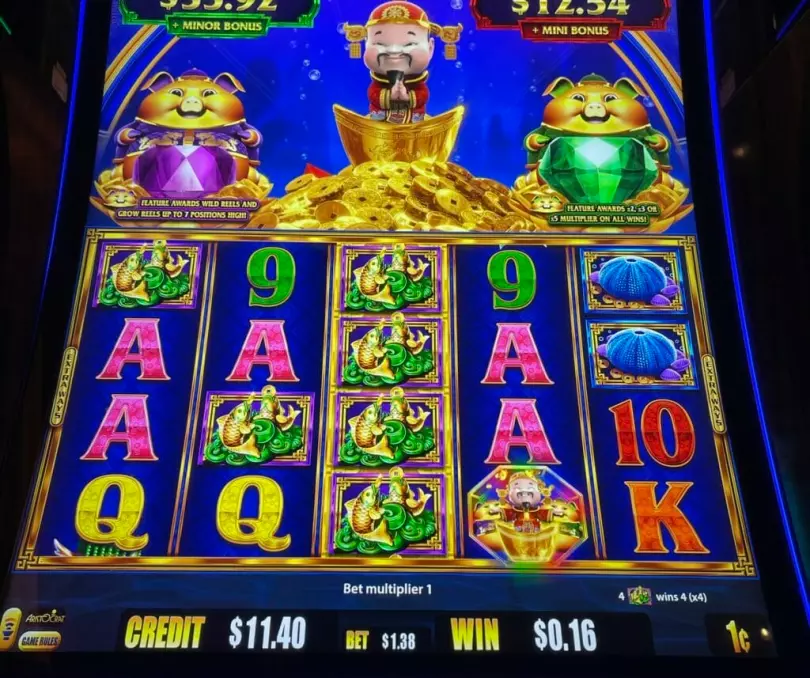
\includegraphics[scale=0.25]{Stacks_Example}
\caption{Photograph of Aristocrat's Gold Stacks 88 Empire Ocean Dragon Slot Machine with a stack of 4 symbols on reel 3 and a stack of 2 symbols on reels 1, 4, and 5.}
\label{goldstacks88}
\end{figure}
\par
Though a common sight to see in any casino, symbol stacking requires more nuance to implement in slot machine math development than the random assortment of symbols that previous research has been built upon.
I believe that if genetic algorithms can yield promising reel strips for slot machine math models with symbol stacking, then perhaps more features for slot machines with unique reel characteristics can be iterated upon via this approach.
\par
I will deviate from previous research in this field by changing the chromosomal representation.
I am re-contextualizing the reel strips as concatenated segments of symbols; a segment may contain at least 1 symbol but it must contain identical symbols.
In other words, I will interpret each stack as a segment of symbols.
\par
This methodology results in a set of reel strips that may vary in length.
Though previous research used the same reel strip length for each reel in a given slot machine, that constraint is uncommon in video slot machine products.
Thus this interpretation may result in more realistic reel strips than what previous research has yielded.
\par
While the chromosomes will still represent reels and still encode non-binary, non-negative numbers, they will represent reel strips as more than just an array of symbols.
The chromosome will be three-dimensional with each column (first dimension) representing a reel in the slot machine model.
The second dimension will be a list of tuples that represents ordered symbol segments; the first element of the tuple is the length of the corresponding segment and the second element is the symbol represented in said segment. 
\begin{figure}[H]
\centering
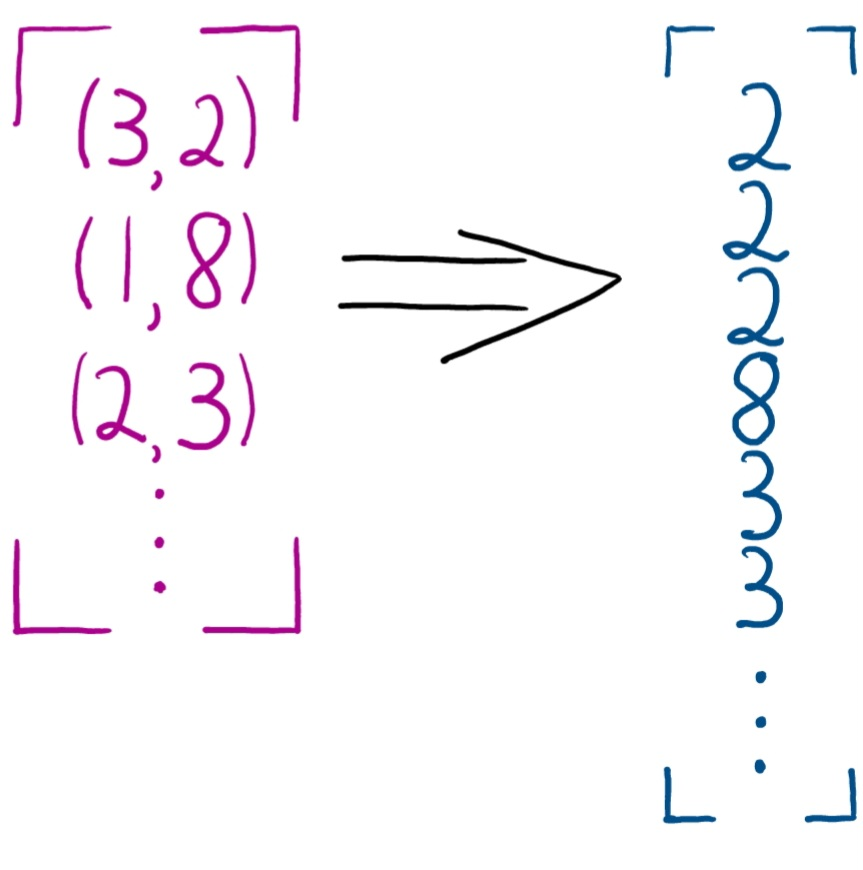
\includegraphics[scale=0.25]{Chromosome_Encoding}
\caption{Example of chromosome encoding and its reel strip decoding.}
\label{encoding}
\end{figure}
I will develop a slot machine paytable that includes lines, win patterns, and a bonus game with a win pattern trigger to evaluate my chromosomes upon.
I plan to program a faster method for calculating RTP for a base game than what Keremedchiev et al. used for their exact RTP approach \cite{keremedchiev2017slot}.
If I fail to develop this method, then each chromosomal evaluation will necessitate between 10,000 and 1,000,000 Monte Carlo simulations.
\par
I plan to use two objective functions for this problem, one to calculate the base game RTP and one to assess the symbol diversity; it is imperative that symbol diversity exists in a slot machine math model that uses symbol stacking, as a symbol is more likely to dominate a given reel strip.
The Fitness function will linearly combine these two objective functions to maximize the RTP to our targeted value.
\par
For this GA I will use a binary tournament for selection and uniform crossover for crossover.
If these methods yield dismal results then I may change my selection and crossover operators as part of my research process.
I plan on utilizing 2 methods for mutation.
First, I plan on swapping two segments in a chromosome selected for mutation.
Second, I plan to randomly mutate tuples in a one of two ways: if a tuple is selected for mutation, then either the size of the segment either increments or decrements by 1, or the symbol will change to either the symbol preceding it or proceeding it in the symbol list.
These mutations are exemplified in Figure \ref{mutation}.
Edge cases for mutation will have special handling as to not construct an illegal chromosome.
\begin{figure}[H]
\centering
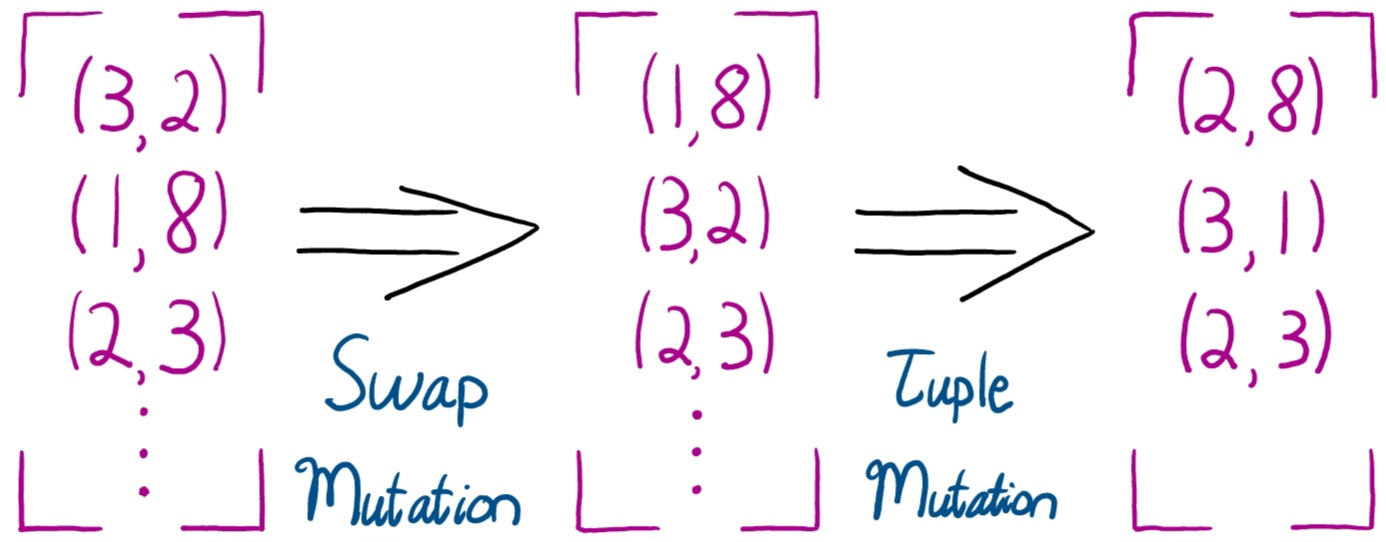
\includegraphics[scale=0.25]{Mutation_Operators}
\caption{Example of chromosome mutation operators.}
\label{mutation}
\end{figure}
\par
I expect to see a diverse set of chromosomes that target our criteria that can serve as viable slot machine models.
I will compare the number of evaluations for convergence to the ones found in previous research to measure the feasibility of this approach.
\section{Summary of Previous Work}
\par
In 2015, Balabanov et. al. published the first paper related to GAs and slot machine RTP optimization\cite{balabanov2015slot}. 
The authors used $100,000$ or $1,000,000$ Monte Carlo simulations to approximate RTP for each individual and they concluded that this method was successful yet time-consuming.
Then again in 2015, Balabanov et al. applied a linear transformation to 3 criteria (RTP, prizes equalization, and symbol diversity) to create a single-objective Discrete Differential Evolution method\cite{balabanovDDE}.
This paper also implemented Monte Carlo simulations for approximating RTP to be used in the objective function for each individual.
While this method mentioned above takes into consideration multiple criteria, it does not examine the tradeoffs made between said criteria.
A paper in 2017 applied the GA approach to optimizing RTP but implemented an exact approach to calculating RTP\cite{keremedchiev2017slot}.
While this approach converged faster than the ones found in the 2015 papers, it took a longer time evaluate an objective function per individual than by using Monte Carlo simulations.
Kamanas et al. implemented Variable Neighborhood Search to attempt to optimize RTP in 2021\cite{kamanas2021slot}.
\printbibliography[title={References}]
\end{document}
